\documentclass[11pt]{article}
\usepackage[parfill]{parskip}
\usepackage{graphicx}
\usepackage{wrapfig}
\usepackage{subcaption}
\usepackage[top=1in, bottom=1in, left=1in, right=1in]{geometry}
\bibliographystyle{plain}
\usepackage{amsmath}
\usepackage{hyperref}
%%%%%%%%%%%%%%%%%%%%%%%%%%%%%%%%%%%%%%%%%%%%%%%%%%%%%%%%%%%%%%%
\usepackage{fancyhdr}
\pagestyle{fancy}
%%% Please add the author's last names
\lhead{Davis, Theriault, Orhai, Westbrook, and Wright}
\rhead{Modeling the World's Systems, 2019}
%%% Please use \cfoot{} to remove page numbers
\cfoot{ }
\renewcommand{\headrulewidth}{0pt}
\renewcommand{\footrulewidth}{0pt}
%%%%%%%%%%%%%%%%%%%%%%%%%%%%%%%%%%%%%%%%%%%%%%%%%%%%%%%%%%%%%%&
\usepackage{titlesec}
\titlespacing{\section}{0pt}{\parskip}{-.5\parskip}
\titlespacing{\subsection}{0pt}{\parskip}{- .5\parskip}
\titlespacing{\subsubsection}{0pt}{\parskip}{- .5\parskip}
\newcommand{\closeup}{\setlength{\itemsep}{-4pt}}

\date{\vspace{-5ex}}
% Use this to get rid of the date

\usepackage{authblk}
\author[1]{Eric Davis}
\author[1]{Alec Theriault}
\author[1]{Max Orhai}
\author[1]{Eddy Westbrook}
\author[1]{Ryan Wright}
\affil[1]{Galois, Inc}

%\setcounter{page}{0}



\title{Machine-Assisted Extraction of Formal Semantics from Domain Specific Semi-Formal Diagrams}

\begin{document}
\maketitle
\vspace{10pt}
\begin{abstract}
Please keep your abstract short, fifteen lines or less.  Remember that the MWS conference is attended by people from many academic disciplines, as well as colleagues in government, industry, foundations and nonprofits, and the defense and intelligence communities.  So strive to make your abstract accessible.
\end{abstract}

\section{Introduction}

\begin{figure}
  \centering
  \begin{subfigure}[b]{0.48\textwidth}
    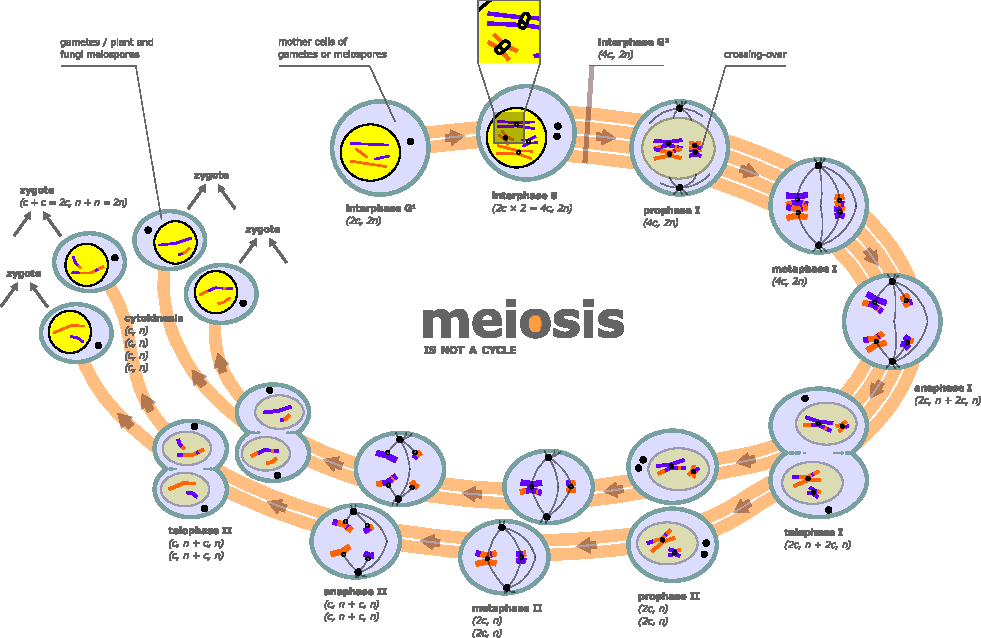
\includegraphics[width=\textwidth]{figs/Diagram_of_meiosis.pdf}
    \caption{Example of a semi-formal diagram of Meoisis. CC-BY-SA 3.0 Marek Kultys, July 2, 2008.}
    \label{Fig:Meiosis}
  \end{subfigure}
  \begin{subfigure}[b]{0.48\textwidth}
    \includegraphics[width=\textwidth]{figs/HIV-Tat-figure.pdf}
    \caption{Example of a semi-formal diagram of the molecular model of the Tat transactivation circuit.}
    \label{Fig:HIV-Tat}
  \end{subfigure}
  \caption{Examples of semi-formal diagrams drawn by domain experts to represent operational semantics and complex
  system models.}
  \label{Fig:Semi-formal}
\end{figure}

"We need to focus more
on how information is managed in living
systems and how this brings about higherlevel biological phenomena. There should be
a concerted programme to investigate this,
which will require both the development of
the appropriate languages to describe information processing in biological systems and
the generation of more effective methods to
translate biochemical descriptions into the
functioning of the logic circuits that underpin
biological phenomena." \cite{nurse2008life}

Abstract machines of systems biology \cite{cardelli2005abstract}

\paragraph{Significance}

\section{Related Work}

Gene gate modeling in the stochastic pi-calculus \cite{blossey2008compositionality}

Pi-calculus \cite{sangiorgi2003pi}

\subsection{Generating Formal Meaning from Informal Diagrams}

\section{AMIDOL}

\begin{figure}
  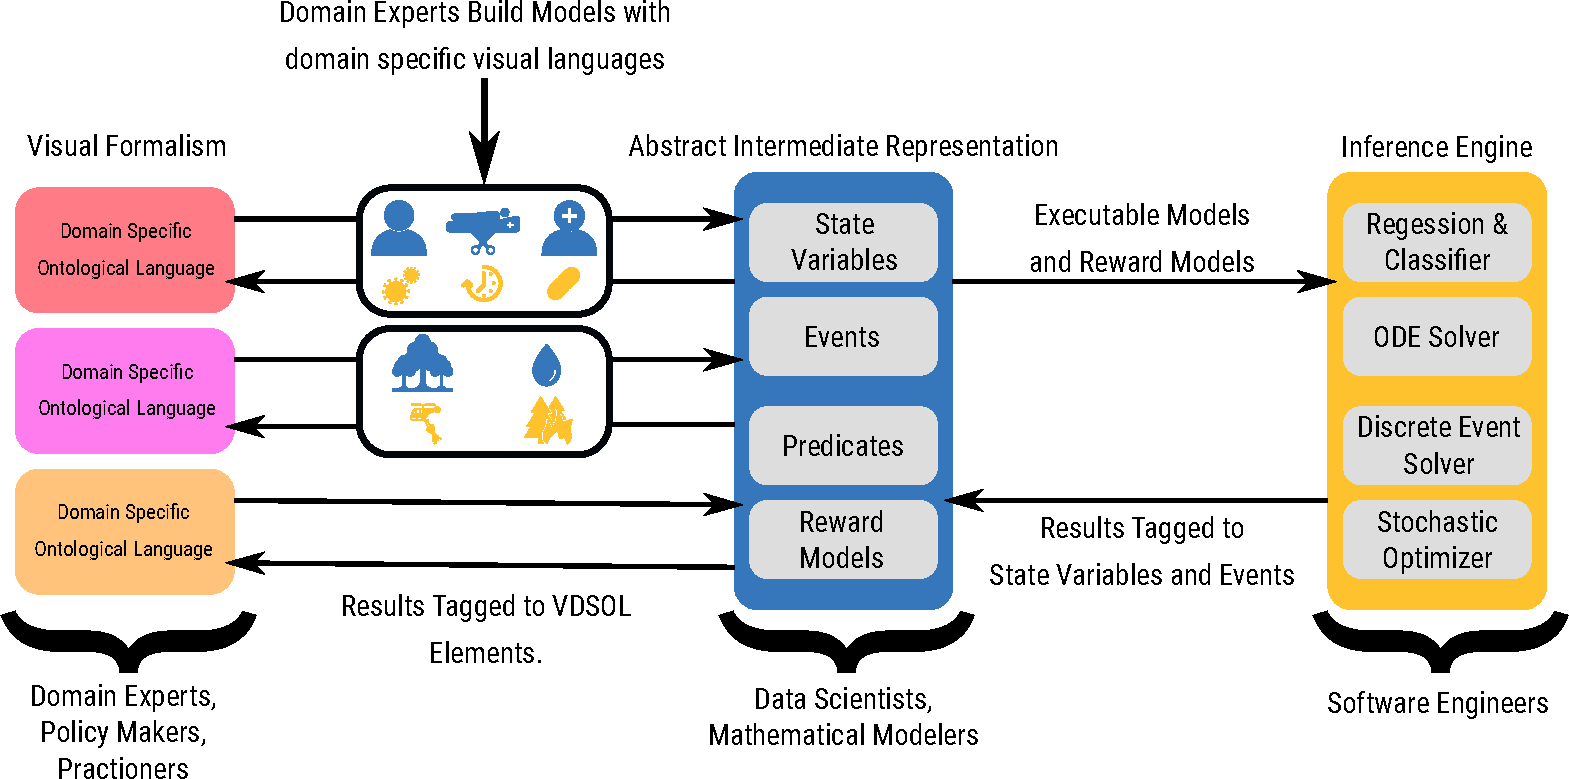
\includegraphics[width=\textwidth]{figs/system-architecture-quad.pdf}
  \caption{AMIDOL Architecture}
\end{figure}

\subsection{Visual Domain Specific Languages}

\subsection{Intermediate Representation}

\paragraph{State and reward variables}

\paragraph{Events}

\paragraph{Input and output predicates}

\subsection{Inference Engine}

\begin{figure}
  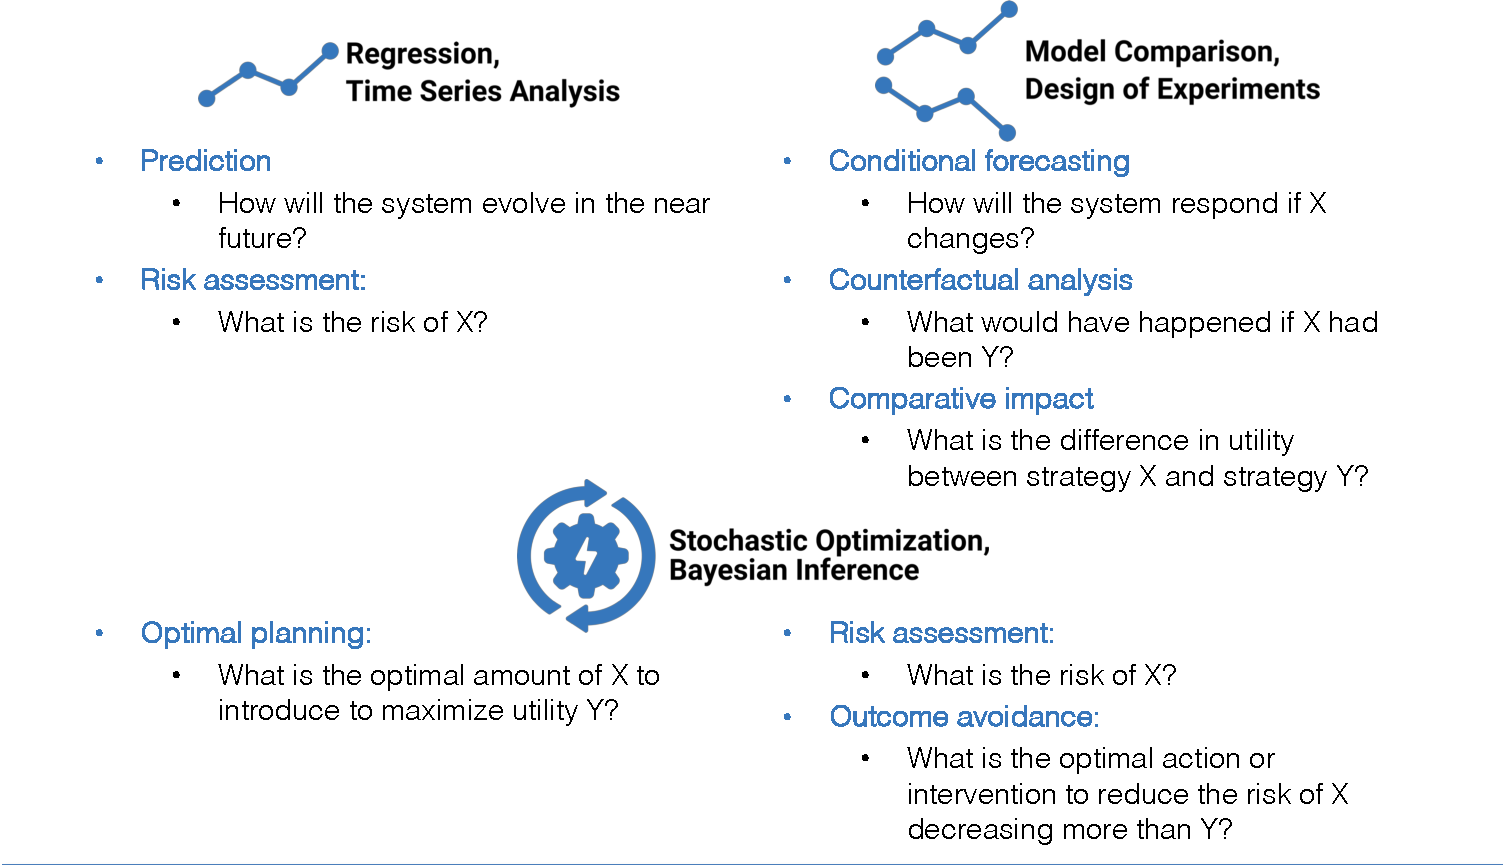
\includegraphics[width=\textwidth]{figs/table.pdf}
  \caption{}
  \label{Fig:InferenceClasses}
\end{figure}

\section{Compartmental Model for Epidemiology}

\subsection{SIRS Model}

H1N1 $R_0$ importance \cite{fraser2009pandemic}.

Ebola $R_0$ importance \cite{fisman2014early}

CDC Data \cite{cdc2019fluview}

\subsection{Vital Dynamics}

\section{Conclusions}

\section{Future Work}

\section{Acknowledgments}

This research has been supported by DARPA contract DARPA-PA-18-02-AIE-FP-039.

\section{Resources, web sites, etc.}

MWS seeks to build a community and share resources, so feel free to have a section in your paper that points readers to web sites, github pages, etc.


%\newcommand*{\doi}[1]{\href{http://dx.doi.org/#1}{doi: #1}}
\bibliography{AMIDOL-MWS}



\end{document}
